\section{Transformadores Densos, Recurrentes y Aumentados con Memoria}
\label{sec:annex-transformer}

Este anexo sintetiza las familias densas, recurrentes y aumentadas con memoria de transformers. El campo ha evolucionado hacia varios paradigmas principales: atención densa global con variantes, compresión de cabezas clave-valor mediante atención por consultas agrupadas, compresión de estado recurrente con decaimiento, modelos de espacio de estado selectivos, integración numérica de profundidad continua, memoria de valores indexada por token y arquitecturas aumentadas con memoria. Comprender esta taxonomía ilumina las compensaciones fundamentales entre expresividad, costo computacional, huella de memoria y simplicidad de despliegue.

\subsection{Atención Densa de Referencia: Estándar, Sigmoide, Continua, Exclusiva y Multi-Token}

\subsubsection{Atención Softmax Estándar}

\begin{figure}[H]
\centering
\fitfigure{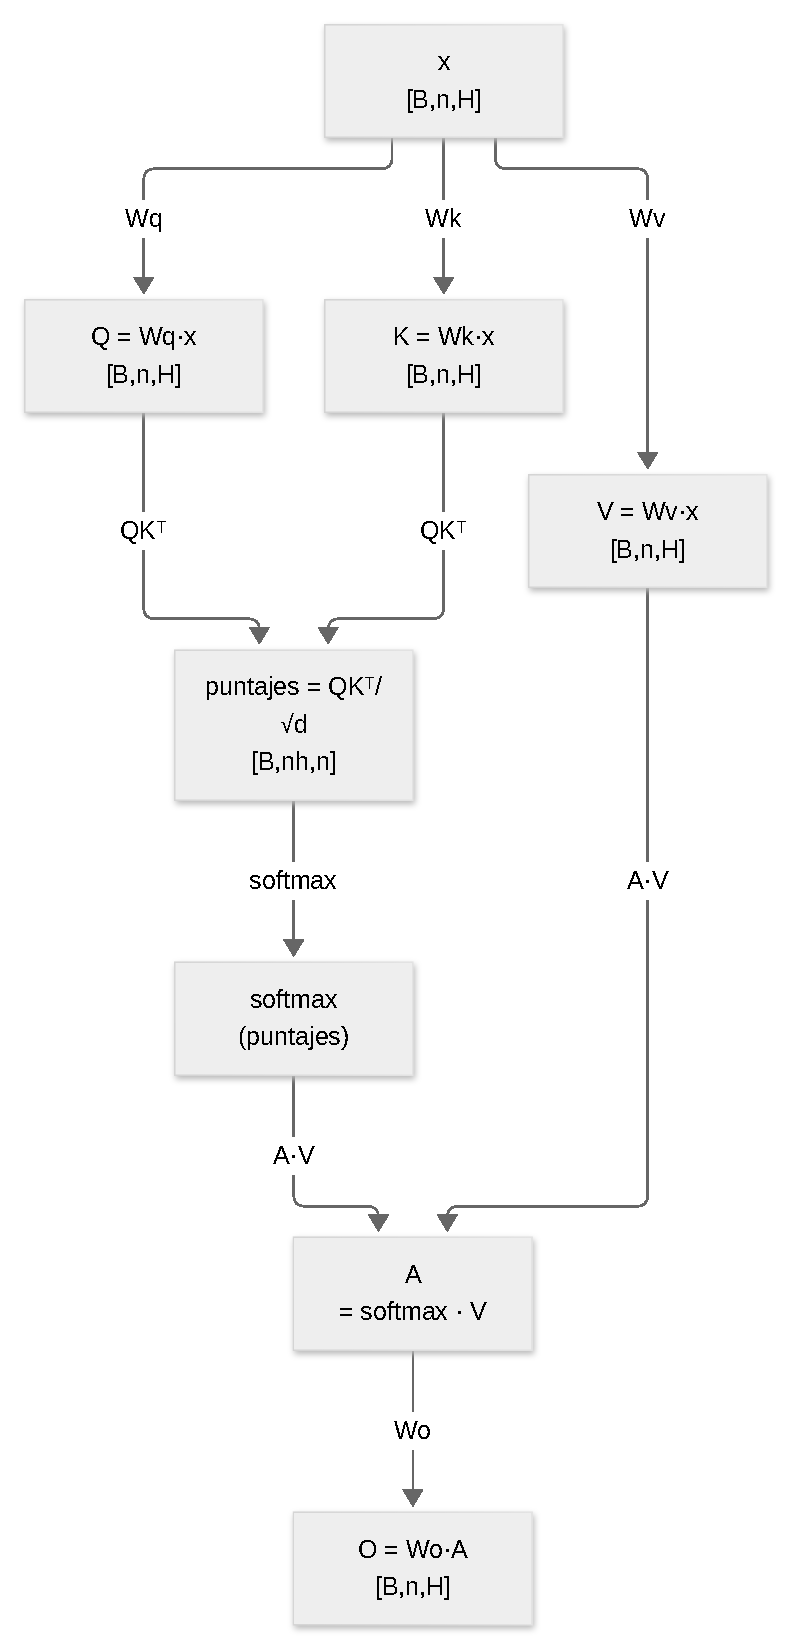
\includegraphics{../paper/figures/mixers/standard-es.pdf}}
\caption{Flujo de datos de la atención softmax estándar: proyecciones Q/K/V paralelas, puntuaciones de producto escalar escaladas, softmax por filas y proyección de salida.}
\label{fig:mixer-standard}
\end{figure}
La atención multi-cabeza estándar \citep{vaswani_attention_2017} calcula la similitud de producto punto escalado entre embeddings de tokens:

\begin{algorithmic}[1]
\State \textbf{Entrada:} Matriz de consulta $\mathbf{Q} \in \mathbb{R}^{n \times d}$, Matriz de clave $\mathbf{K} \in \mathbb{R}^{n \times d}$, Matriz de valor $\mathbf{V} \in \mathbb{R}^{n \times d}$
\State $\text{puntajes} \gets \frac{\mathbf{Q}\mathbf{K}^\top}{\sqrt{d}} \in \mathbb{R}^{n \times n}$ \Comment{calcular similitudes por pares}
\State $\text{pesos\_atencion} \gets \texttt{softmax}(\text{puntajes}, \text{eje}=1) \in \mathbb{R}^{n \times n}$ \Comment{normalizar sobre las claves}
\State \textbf{Salida:} $\mathbf{Y} = \text{pesos\_atencion} \cdot \mathbf{V} \in \mathbb{R}^{n \times d}$ \Comment{combinación ponderada de valores}
\end{algorithmic}

Para generación autorregresiva, el almacenamiento en caché KV guarda claves y valores pasados para evitar el recálculo $\mathcal{O}(n^2)$. Sin embargo, este caché de crecimiento lineal ocupa $\sim n \cdot d_{\text{oculto}}$ bytes, lo que puede consumir cientos de gigabytes para modelos de miles de millones de parámetros. La atención estándar logra una \textbf{expresividad perfecta} dentro de la ventana de contexto---cualquier token puede atender a cualquier otro token con pesos aprendidos---pero paga el precio del cómputo denso.

\begin{itemize}[leftmargin=*]
    \item \textbf{Complejidad de entrenamiento}: $\mathcal{O}(n^2 \cdot d)$ tiempo, $\mathcal{O}(n^2)$ espacio (materialización de la matriz de atención).
    \item \textbf{Complejidad de inferencia}: $\mathcal{O}(n)$ tiempo por token, $\mathcal{O}(n)$ espacio (caché KV).
    \item \textbf{Fortalezas}: Expresividad incomparable; recuperación perfecta del historial; altamente paralelizable.
    \item \textbf{Debilidades}: El cuello de botella cuadrático prohíbe contextos muy largos; el caché KV domina la memoria durante la generación.
\end{itemize}

\subsubsection{Atención Sigmoide}

\begin{figure}[H]
\centering
\fitfigure{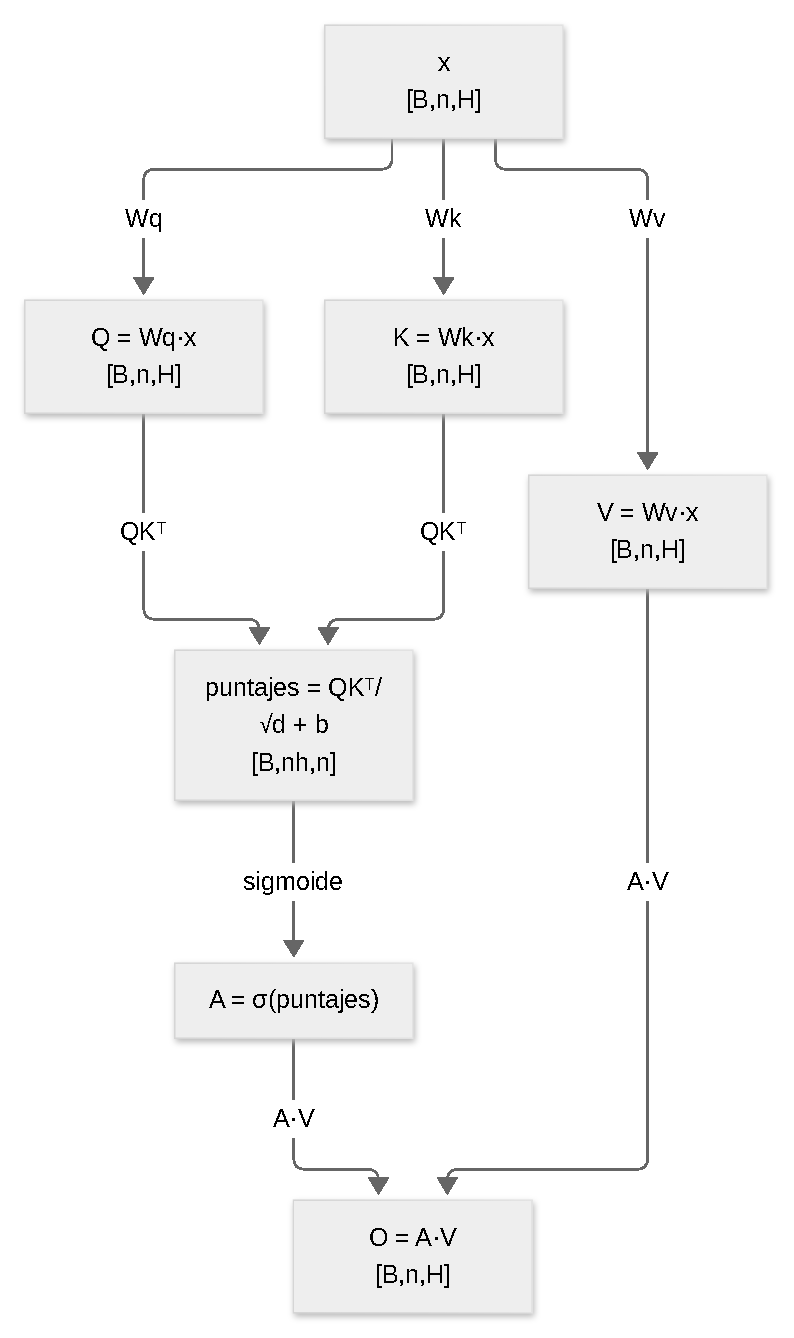
\includegraphics{../paper/figures/mixers/sigmoid-es.pdf}}
\caption{Flujo de datos de la atención sigmoide: una sigmoide elemento a elemento sustituye al softmax por filas, de modo que los pesos de atención no tienen por qué sumar uno.}
\label{fig:mixer-sigmoid}
\end{figure}
La atención sigmoide reemplaza el softmax por filas con una activación sigmoide elemento a elemento \citep{ramapuram_theory_2024}:

\begin{algorithmic}[1]
\State \textbf{Entrada:} $\mathbf{Q}, \mathbf{K}, \mathbf{V}$ como arriba, sesgo aprendible $\mathbf{b} \in \mathbb{R}^{n \times n}$
\State $\text{logits} \gets \frac{\mathbf{Q}\mathbf{K}^\top}{\sqrt{d}} + \mathbf{b}$
\State $\text{pesos\_atencion} \gets \sigma(\text{logits})$ \Comment{sigmoide elemento a elemento, no softmax}
\State \textbf{Salida:} $\mathbf{Y} = \text{pesos\_atencion} \odot \mathbf{V}$
\end{algorithmic}

A diferencia de softmax, la sigmoide no impone una distribución de probabilidad (los pesos no necesitan sumar 1), lo que permite una independencia de tokens más fuerte. El análisis teórico mediante mezcla de expertos muestra que la sigmoide alcanza una complejidad muestral superior: convergencia $\mathcal{O}(n^{-0.51})$ para expertos ReLU frente a $\mathcal{O}(n^{-0.24})$ de softmax. Sin embargo, el entrenamiento empírico reveló inestabilidades de gradiente a escala. El remedio es la \textbf{norma híbrida}---agregar normalización después de la salida de atención---que estabiliza los gradientes sin sacrificar los beneficios teóricos del enrutamiento elemento a elemento.

\begin{itemize}[leftmargin=*]
    \item \textbf{Complejidad de entrenamiento}: $\mathcal{O}(n^2 \cdot d)$ (idéntico al estándar), pero las operaciones elemento a elemento permiten una aceleración de inferencia del 17\% mediante FlashSigmoid.
    \item \textbf{Complejidad de inferencia}: $\mathcal{O}(n)$ por token con caché KV (asintóticamente igual, pero con factores constantes más bajos).
    \item \textbf{Fortalezas}: Supera la competencia de suma cero; evita la sincronización por filas; implementación eficiente en hardware.
    \item \textbf{Debilidades}: Requiere estabilización cuidadosa (norma híbrida); inestabilidad de entrenamiento a grandes escalas sin pérdida auxiliar.
\end{itemize}

\subsubsection{Atención por Consultas Agrupadas (GQA)}

\begin{figure}[H]
\centering
\fitfigure{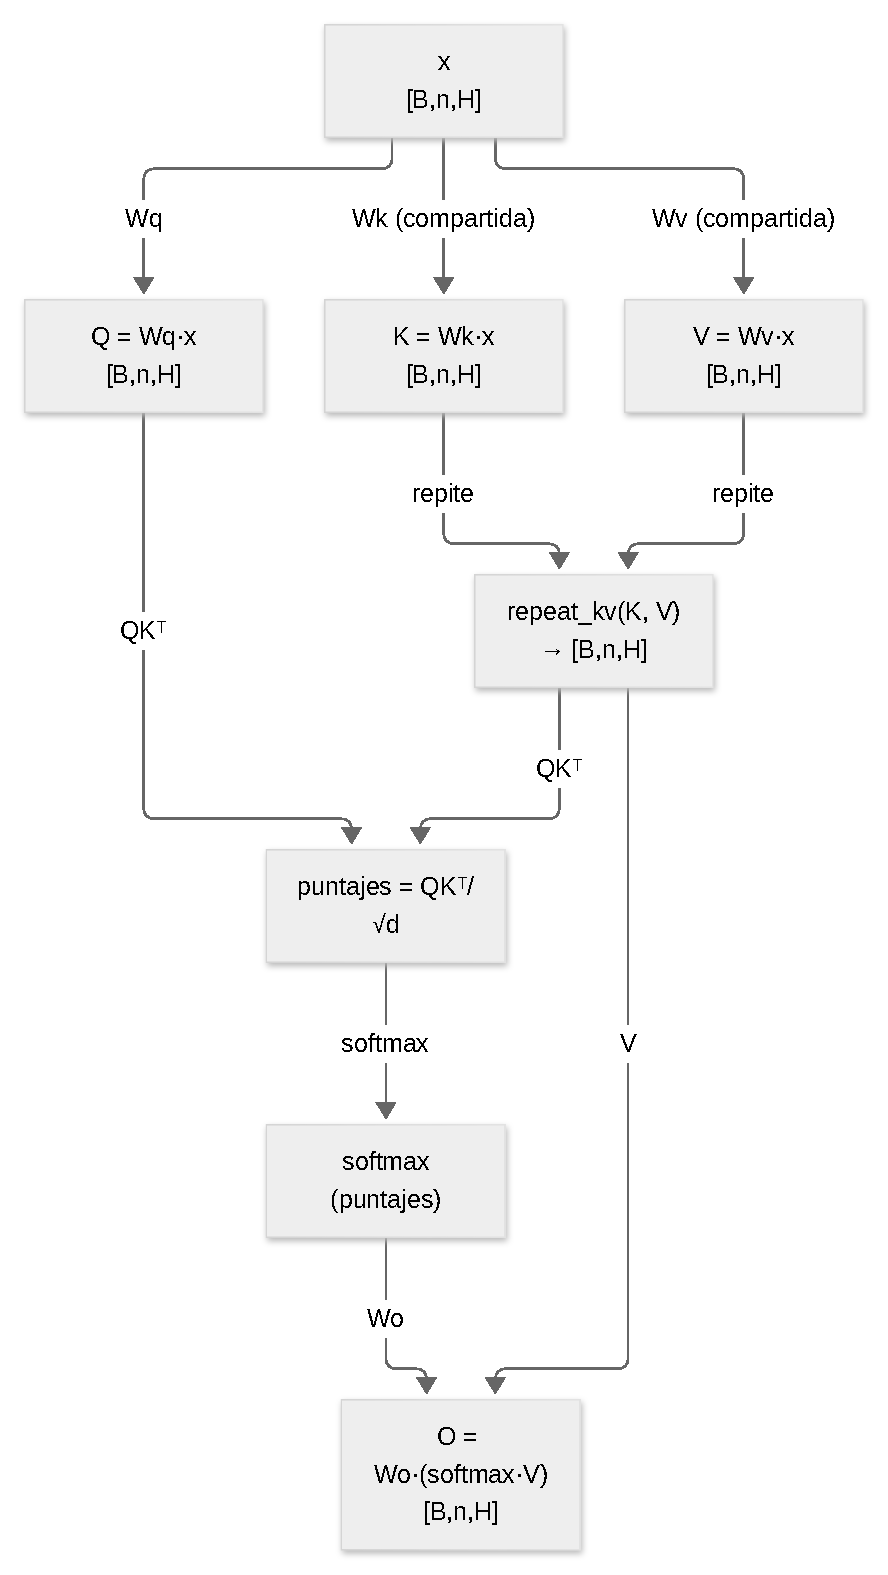
\includegraphics{../paper/figures/mixers/gqa-es.pdf}}
\caption{Flujo de datos de la atención por consultas agrupadas: las claves y los valores se proyectan a menos cabezas, se expanden mediante repetición entrelazada y se comparten en cada grupo de cabezas de consulta.}
\label{fig:mixer-gqa}
\end{figure}
La atención por consultas agrupadas (GQA) \citep{ainslie_gqa_2023} tiende un puente entre la atención multi-cabeza (MHA) y la atención multi-consulta (MQA) al particionar las cabezas de consulta en grupos, cada uno compartiendo una sola cabeza clave-valor. Si $h$ es el número total de cabezas de atención, $h_k$ es el número de cabezas clave-valor, y $G = h / h_k$ es el tamaño del grupo, entonces cada grupo de $G$ cabezas de consulta comparte una cabeza KV:

\begin{algorithmic}[1]
\State \textbf{Entrada:} $\mathbf{Q} \in \mathbb{R}^{n \times h \cdot d_h}$, $\mathbf{K} \in \mathbb{R}^{n \times h_k \cdot d_h}$, $\mathbf{V} \in \mathbb{R}^{n \times h_k \cdot d_h}$
\State $\mathbf{K}_{\text{completo}} \gets \texttt{repeat\_interleave}(\mathbf{K}, G)$ \Comment{expandir de $h_k$ a $h$ cabezas}
\State $\mathbf{V}_{\text{completo}} \gets \texttt{repeat\_interleave}(\mathbf{V}, G)$
\State $\text{puntajes} \gets \frac{\mathbf{Q}\mathbf{K}_{\text{completo}}^\top}{\sqrt{d_h}} \in \mathbb{R}^{n \times n}$ \Comment{producto punto estándar tras expansión}
\State $\text{pesos\_atencion} \gets \texttt{softmax}(\text{puntajes}, \text{eje}=1)$
\State \textbf{Salida:} $\mathbf{Y} = \text{pesos\_atencion} \cdot \mathbf{V}_{\text{completo}} \in \mathbb{R}^{n \times h \cdot d_h}$
\end{algorithmic}

GQA interpola suavemente entre MHA ($h_k = h$, $G = 1$) y MQA ($h_k = 1$, $G = h$). La ventaja clave es un balance ajustable entre la huella del caché KV y la capacidad representacional. Cada cabeza KV adicional consume $2 \cdot d_h \cdot n$ bytes extra en el caché, por lo que reducir $h_k$ produce ahorros proporcionales de memoria.

\begin{itemize}[leftmargin=*]
    \item \textbf{Complejidad de entrenamiento}: $\mathcal{O}(n^2 \cdot h \cdot d_h)$ (idéntico a MHA tras la expansión de cabezas).
    \item \textbf{Complejidad de inferencia}: $\mathcal{O}(n)$ por token, espacio de caché KV $\mathcal{O}(h_k \cdot n \cdot d_h)$.
    \item \textbf{Fortalezas}: Balance flexible de cabezas; probado a escala (Llama 2 y 3 usan $h_k = 8$ cabezas KV con $h = 32$ cabezas de consulta); reduce el caché KV en factor $G \times$; soporta inferencia rápida con FlashAttention.
    \item \textbf{Debilidades}: Menos cabezas KV pueden reducir la capacidad representacional en modelos pequeños; requerir que $h_k$ divida a $h$ restringe las opciones arquitectónicas.
\end{itemize}

\subsubsection{Atención Continua}

\begin{figure}[H]
\centering
\fitfigure{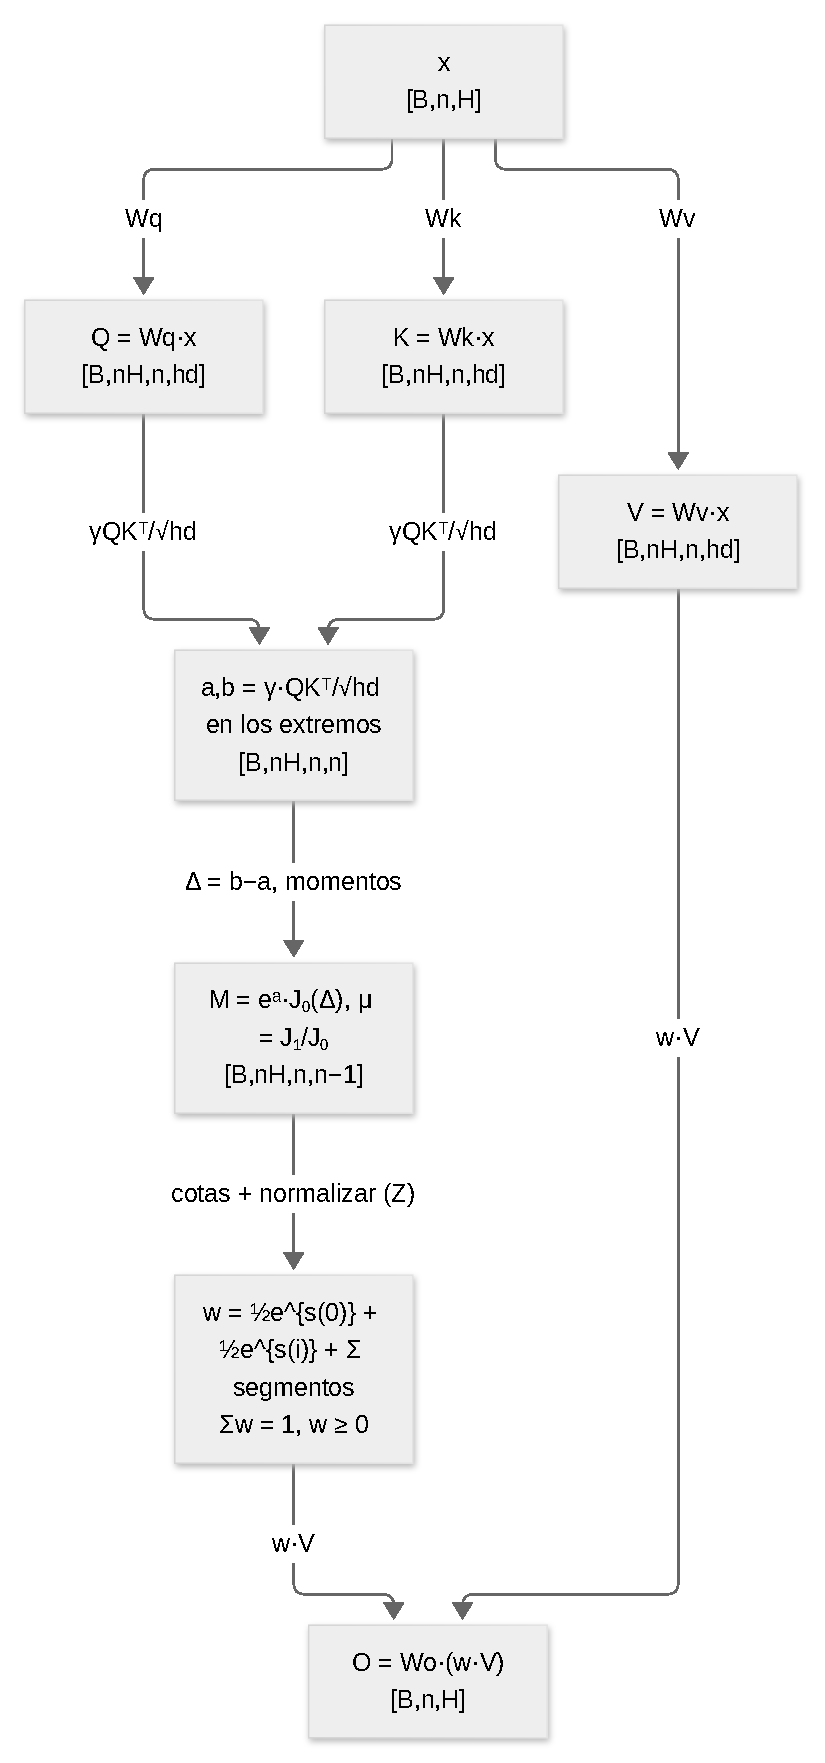
\includegraphics{../paper/figures/mixers/ca-es.pdf}}
\caption{Flujo de datos de la Atención Continua: puntajes de extremo de la trayectoria lineal de claves, integración exacta por tramos mediante momentos exponenciales, extensiones de medio token en los bordes y pesos efectivos normalizados sobre los valores originales.}
\label{fig:mixer-ca-es}
\end{figure}
La Atención Continua \citep{khadangi_continuum_2026} reemplaza la recuperación softmax discreta por la integración exacta sobre una trayectoria de memoria continua, lineal por tramos. Las claves y valores adyacentes se interpolan de modo que $\mathbf{k}(t)$ y $\mathbf{v}(t)$ quedan definidos en toda posición del dominio visible:
\begin{equation}
\mathbf{k}_j(u) = (1-u)\,\mathbf{k}_{j-1} + u\,\mathbf{k}_j, \qquad
\mathbf{v}_j(u) = (1-u)\,\mathbf{v}_{j-1} + u\,\mathbf{v}_j,
\end{equation}
con $u = t-(j-1)\in[0,1]$ en el intervalo $[j-1,j]$; extensiones constantes de medio token cubren $[-1/2,0]$ y $[i,i+1/2]$. Cada consulta induce una densidad de relevancia exponencial sobre su prefijo visible,
\begin{equation}
s_i(t) = \frac{\gamma}{\sqrt{d_h}}\,\mathbf{q}_i^\top \mathbf{k}(t), \qquad
p_i(t) = \frac{\exp(s_i(t))}{Z_i}, \qquad
\mathbf{o}_i = \int_{-1/2}^{i+1/2} p_i(t)\,\mathbf{v}(t)\,dt,
\end{equation}
donde $\gamma>0$ es la ganancia de puntaje ($\gamma=1/\tau$). Como la trayectoria de claves es lineal dentro de cada tramo, el puntaje es afín, $s_{ij}(u) = a_{ij} + u\,\Delta_{ij}$ con $a_{ij}=s_i(j-1)$, $b_{ij}=s_i(j)$ y $\Delta_{ij}=b_{ij}-a_{ij}$, de modo que las integrales tienen forma cerrada en los momentos exponenciales $J_n(\Delta)=\int_0^1 u^n e^{\Delta u}\,du$:
\begin{align}
J_0(\Delta) &= \frac{e^{\Delta}-1}{\Delta}, \qquad
J_1(\Delta) = \frac{(\Delta-1)e^{\Delta}+1}{\Delta^2}, \\
M_{ij} &= e^{a_{ij}} J_0(\Delta_{ij}), \qquad
\mathbf{U}_{ij} = e^{a_{ij}}\big[(J_0-J_1)\,\mathbf{v}_{j-1} + J_1\,\mathbf{v}_j\big], \\
Z_i &= \tfrac12 e^{s_i(0)} + \tfrac12 e^{s_i(i)} + \sum_{j=1}^{i} M_{ij}, \qquad
\mathbf{o}_i = \frac{\mathbf{U}_i^{\mathrm{cap}} + \sum_{j=1}^{i}\mathbf{U}_{ij}}{Z_i},
\end{align}
con $\mu(\Delta)=J_1/J_0$ la posición de recuperación normalizada dentro de un tramo. Como las contribuciones no son negativas, la atención continua equivale a una suma ponderada normalizada y no negativa de los valores originales, $\mathbf{o}_i = \sum_{j\le i} w_{ij}\mathbf{v}_j$ con $w_{ij}\ge 0$ y $\sum_j w_{ij}=1$; puntajes visibles iguales se reducen exactamente a atención causal uniforme y $o_0=v_0$. La variante con ganancia aprendida añade un escalar por cabeza ($\gamma=\exp(\rho)$, inicializada en $\gamma=1$ en el modelo de 101M; la variante fija CA-P usa $\gamma=1/0.30$ y no añade parámetros). La forma encoder (bidireccional) integra sobre la trayectoria completa $[-1/2,n-1/2]$ --- la extensión simétrica natural del artículo, que sólo define el caso causal.

\begin{algorithmic}[1]
\State \textbf{Entrada:} $\mathbf{Q}, \mathbf{K}, \mathbf{V} \in \mathbb{R}^{n \times d_h}$, ganancia $\gamma>0$
\State $\mathbf{S} \gets \gamma\,\mathbf{Q}\mathbf{K}^\top/\sqrt{d_h}$ \Comment{puntajes de extremo, Ec. (4)}
\State enmascarar $\mathbf{S}$ al prefijo visible; restar el máximo de fila $m$ (estabilidad)
\State $\Delta_{ij} \gets \mathbf{S}_{j}-\mathbf{S}_{j-1}$; \quad $J_0,J_1 \gets$ Ecs. (11)--(12) (serie cerca de $\Delta=0$)
\State $M_{ij} \gets e^{a_{ij}-m}J_0$, \quad $w^{(L)}_{ij}\gets M_{ij}(1-\mu)$, \quad $w^{(R)}_{ij}\gets M_{ij}\mu$
\State sumar las extensiones de medio token $\tfrac12 e^{s_i(0)-m}$ y $\tfrac12 e^{s_i(i)-m}$; normalizar por $Z_i$
\State \textbf{Salida:} $\mathbf{o}_i = \sum_{j\le i} w_{ij}\mathbf{v}_j$ \Comment{Ec. (24)}
\end{algorithmic}

\begin{itemize}[leftmargin=*]
    \item \textbf{Complejidad de entrenamiento}: $\mathcal{O}(n^2 d)$ --- idéntica al softmax denso; los momentos en forma cerrada reemplazan al softmax (sin cuadratura).
    \item \textbf{Complejidad de inferencia}: $\mathcal{O}(n)$ por token con caché KV; los pesos efectivos se recalculan localmente por fila sobre el prefijo cacheado en cada paso (exacto).
    \item \textbf{Fortalezas}: Recuperación continua exacta con pesos efectivos normalizados no negativos; cero parámetros más allá de las proyecciones en la forma de ganancia fija; resultados multilingües y zero-shot sólidos (macro FLORES 1.8915 BPB, una reducción del 5.8\% frente al mejor baseline y el mejor puntaje en todos los idiomas; HellaSwag y ARC-Challenge los mejores entre los baselines); 42\% menos bytes de entrenamiento para alcanzar el umbral de 1.10 BPB que un Transformer emparejado.
    \item \textbf{Debilidades}: La aritmética cuadrática de atención persiste; el desempeño en código fuente es el más débil de las cinco arquitecturas (Stack-smol 3.3451 BPB); robustez reducida a la eliminación de bytes y a perturbaciones ``antspeak''.
\end{itemize}

\subsubsection{Atención Exclusiva (XSA)}

\begin{figure}[H]
\centering
\fitfigure{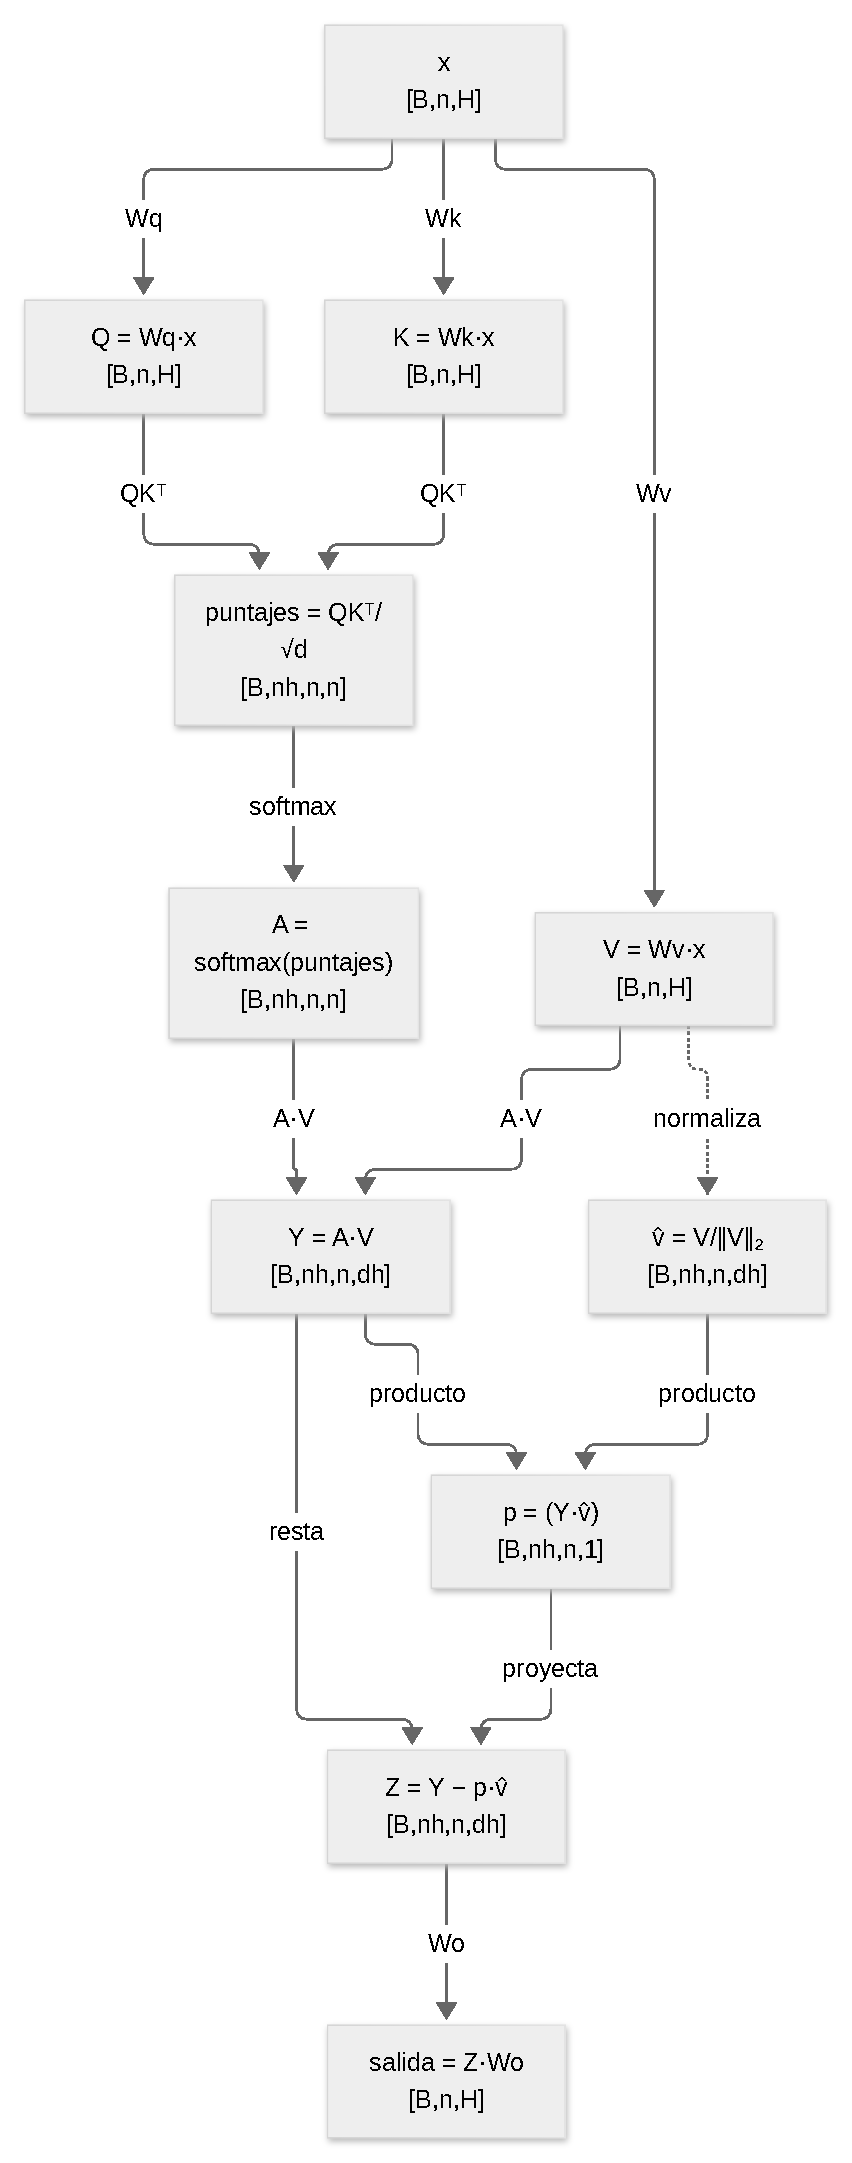
\includegraphics{../paper/figures/mixers/xsa-es.pdf}}
\caption{Flujo de datos de la Atención Exclusiva: la salida estándar de atención softmax $Y$, la normalización del vector de valor propio del token y la resta de la proyección $p=(Y\cdot\hat v)$, de modo que la salida de la cabeza no conserva componente alguna en la dirección del valor propio.}
\label{fig:mixer-xsa-es}
\end{figure}
La Atención Exclusiva (XSA, \emph{Exclusive Self Attention}) \citep{zhai_exclusive_2026} parte de la observación de que, en Transformers entrenados, la salida de atención $\mathbf{y}_i$ conserva una alta similitud coseno con el vector de valor propio del token $\mathbf{v}_i$ ---el \emph{sesgo de similitud de atención}--- y que esa similitud crece con la profundidad. Dado que la ruta residual y la FFN posterior ya transportan la información puntual de la posición $i$, esa componente es redundante y compite con el trabajo real de la capa: modelar contexto. XSA la elimina explícitamente. La primera línea es atención softmax causal estándar:
\begin{equation}
\mathbf{q}_i = \mathbf{W}_q\mathbf{x}_i, \quad
\mathbf{k}_j = \mathbf{W}_k\mathbf{x}_j, \quad
\mathbf{v}_j = \mathbf{W}_v\mathbf{x}_j, \quad
a_{i,j} = \frac{\exp(\mathbf{q}_i^\top\mathbf{k}_j)}{\sum_{j'=1}^{i}\exp(\mathbf{q}_i^\top\mathbf{k}_{j'})}, \quad
\mathbf{y}_i = \sum_{j=1}^{i} a_{i,j}\mathbf{v}_j,
\end{equation}
y el paso exclusivo proyecta la salida ortogonalmente fuera de la dirección del valor propio:
\begin{equation}
\hat{\mathbf{v}}_i = \frac{\mathbf{v}_i}{\|\mathbf{v}_i\|_2}, \qquad
\mathbf{z}_i = \mathbf{y}_i - \big(\mathbf{y}_i^\top \hat{\mathbf{v}}_i\big)\,\hat{\mathbf{v}}_i .
\end{equation}
El paso no tiene parámetros, es local a la fila (solo consume el valor del token actual) y es diferenciable, por lo que se entrena de extremo a extremo con las cuatro proyecciones habituales $\mathbf{W}_q,\mathbf{W}_k,\mathbf{W}_v,\mathbf{W}_o \in \mathbb{R}^{H\times H}$; el conteo de parámetros es exactamente $4H^2$, idéntico al de la atención estándar. Eliminar la dirección propia puede leerse como un sumidero de atención implícito: la masa no deseada se estaciona en la diagonal $a_{i,i}$ y luego se descarta, lo que es coherente con la robustez observada frente a tokens sumidero explícitos.

\begin{algorithmic}[1]
\State \textbf{Entrada:} $\mathbf{x}$; $\mathbf{W}_q,\mathbf{W}_k,\mathbf{W}_v,\mathbf{W}_o$; $n_h$ cabezas de ancho $d_h$
\State $\mathbf{Q}\gets\mathbf{x}\mathbf{W}_q$, $\mathbf{K}\gets\mathbf{x}\mathbf{W}_k$, $\mathbf{V}\gets\mathbf{x}\mathbf{W}_v$ \Comment{reformar por cabeza}
\State $\mathbf{Y} \gets \texttt{softmax}(\mathbf{Q}\mathbf{K}^\top/\sqrt{d_h} + \text{máscara causal})\,\mathbf{V}$ \Comment{SDPA estándar}
\State $\hat{\mathbf{V}} \gets \mathbf{V} / \|\mathbf{V}\|_2$ \Comment{por fila y por cabeza}
\State $\mathbf{Z} \gets \mathbf{Y} - (\mathbf{Y}\odot\hat{\mathbf{V}})\text{-suma}_{d_h}\cdot\hat{\mathbf{V}}$ \Comment{paso XSA, Eq. (2)}
\State \textbf{Salida:} $\mathbf{Z}\mathbf{W}_o$
\end{algorithmic}

\begin{itemize}[leftmargin=*]
    \item \textbf{Complejidad de entrenamiento}: $\mathcal{O}(n^2 d)$ --- domina la atención softmax; la exclusión es $\mathcal{O}(nd)$ y se mide como sobrecosto mínimo (las curvas de velocidad y memoria se solapan con la línea base en distintas longitudes de secuencia y anchos de modelo).
    \item \textbf{Complejidad de inferencia}: $\mathcal{O}(n)$ por token con una caché KV simple; la exclusión solo lee $\mathbf{v}_i$ recién calculado, por lo que la decodificación incremental es exacta (clase (i)).
    \item \textbf{Fortalezas}: Cero parámetros adicionales; cambio de dos líneas; ganancias consistentes de entrenamiento/validación con 0.7B, 1.3B y 2.7B parámetros en FineWeb-100BT (+0.26, +1.03 y +1.36 puntos promedio en tareas posteriores frente a SA); el margen crece con la longitud de secuencia (512 a 16k) y es estable entre tasas de aprendizaje y configuraciones de sumideros de atención.
    \item \textbf{Debilidades}: La evidencia es solo de modelado de lenguaje; el artículo no ofrece fundamento teórico más allá de la motivación empírica; la normalización L2 por token es un kernel extra (pequeño) frente a SDPA vanilla; la variante de codificador (bidireccional) que usa este toolkit es una extensión agnóstica a la máscara de la formulación causal del artículo.
\end{itemize}

\subsubsection{Atención Multi-Token (MTA)}

\begin{figure}[H]
\centering
\fitfigure{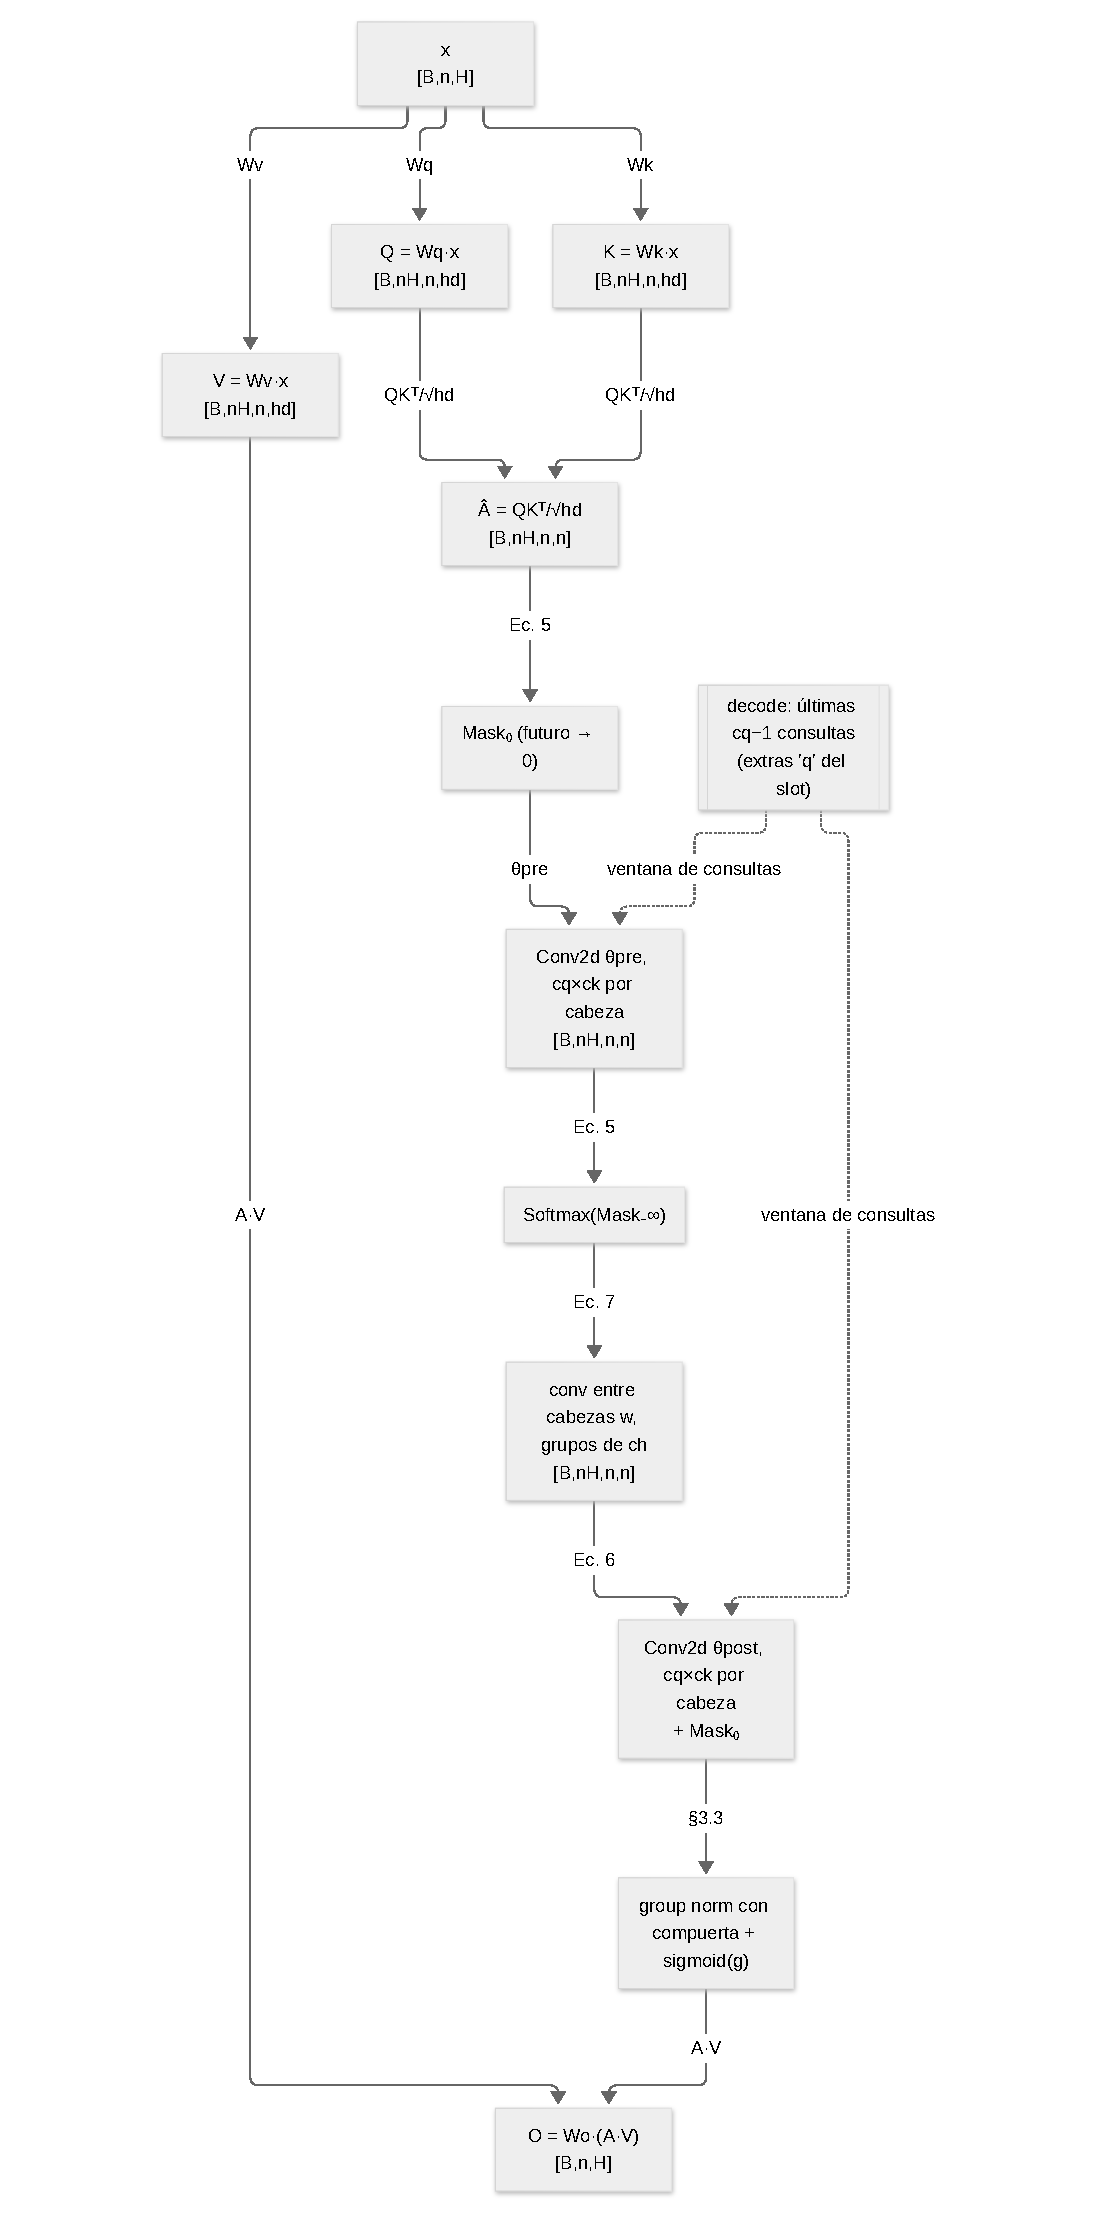
\includegraphics{../paper/figures/mixers/mta-es.pdf}}
\caption{Flujo de datos de la Atención Multi-Token: convolución causal consulta-clave sobre el mapa de puntajes (pre-softmax, Eq.~\ref{eq:mta-pre-es}), softmax, convolución de mezcla de cabezas por grupos (Eq.~\ref{eq:mta-head-es}), una segunda convolución consulta-clave post-softmax y la normalización de grupo con compuerta antes de la proyección de salida; la ruta punteada es la cola de consultas en decodificación.}
\label{fig:mixer-mta-es}
\end{figure}
La Atención Multi-Token \citep{golovneva_multi_token_2025} ataca el \emph{cuello de botella de un solo token} de la atención softmax: cada peso $a_{ij}$ se decide con una sola consulta y una sola clave, de modo que una región del contexto identificada por varios tokens (una oración que menciona a ``Alice'' y a ``rabbit'') debe comprimirse en un único vector. MTA conserva el esqueleto cuadrático de la atención y hace interactuar a consultas, claves y cabezas vecinas mediante pequeñas convoluciones aprendidas sobre el mapa de puntajes. La convolución consulta-clave mezcla los logits de una ventana de $c_q$ consultas y $c_k$ claves, por cabeza:
\begin{equation}
a_{ij} = \operatorname{Softmax}\Big(\sum_{i'=0}^{c_q-1}\ \sum_{j'=-\lfloor c_k/2\rfloor}^{\lceil c_k/2\rceil-1}
\mathbf{1}_{i\ge j-j'}\ \theta_{i',j'}\ \mathbf{q}_{i-i'}\mathbf{k}_{j-j'}^{\top}/\sqrt{d_h}\Big),
\label{eq:mta-exact-es}
\end{equation}
y, como ese indicador exigiría núcleos CUDA a medida, la implementación por defecto aplica dos veces la máscara causal existente:
\begin{equation}
\mathbf{A} = \operatorname{Softmax}\Big(\operatorname{Mask}_{-\infty}\big(\operatorname{Conv2d}_{\theta}(\operatorname{Mask}_{0}(\hat{\mathbf{A}}))\big)\Big),
\qquad
\mathbf{A} = \operatorname{Mask}_{0}\Big(\operatorname{Conv2d}_{\theta}\big(\operatorname{Softmax}(\operatorname{Mask}_{-\infty}(\hat{\mathbf{A}}))\big)\Big),
\label{eq:mta-pre-es}
\end{equation}
donde la primera expresión es la variante pre-softmax (la predeterminada del paper) y la segunda la post-softmax (interacción aditiva en lugar de multiplicativa); por defecto se aplican ambas. La mezcla de cabezas divide las $n_h$ cabezas en $n_h/c_h$ grupos sin solapamiento y mezcla cada grupo con su propio núcleo $c_h\times c_h$,
\begin{equation}
\mathbf{A}^{1}_{\text{new}} = w_{11}\mathbf{A}^{1}+w_{12}\mathbf{A}^{2}, \qquad
\mathbf{A}^{2}_{\text{new}} = w_{21}\mathbf{A}^{1}+w_{22}\mathbf{A}^{2},
\label{eq:mta-head-es}
\end{equation}
de modo que los mapas de atención se combinan entre cabezas (una mezcla post-softmax $2\times2$ equivale a duplicar el rango de las proyecciones de valor/salida, Apéndice~B del paper). Finalmente, una normalización por grupos sobre cada conjunto de $c_h$ cabezas seguida de una compuerta sigmoide por cabeza, $\operatorname{diag}(\sigma(\mathbf{g}))\operatorname{GroupNorm}(\mathbf{A}\mathbf{V})$, contrarresta la corriente residual y permite encender o apagar cabezas según la capa; el paper reporta 10.90 de perplejidad de validación con compuerta escalar frente a 11.03 sin escalado y 11.41 con escalado layer-norm. Los núcleos se inicializan en la identidad (la opción que mejor converge) y el mixer añade solo cerca del $0.001\%$ de los parámetros a escala 880M: $n_h(2c_qc_k + c_h) + 2H + n_h$, es decir, un escalar por cabeza para la compuerta, una normalización de grupo afín y los núcleos.

\begin{algorithmic}[1]
\State \textbf{Entrada:} $\mathbf{x}$; $\mathbf{W}_q,\mathbf{W}_k,\mathbf{W}_v,\mathbf{W}_o$; hiperparámetros $c_q,c_k,c_h$
\State $\mathbf{Q}\gets\mathbf{x}\mathbf{W}_q$, $\mathbf{K}\gets\mathbf{x}\mathbf{W}_k$, $\mathbf{V}\gets\mathbf{x}\mathbf{W}_v$; $\hat{\mathbf{A}}\gets\mathbf{Q}\mathbf{K}^\top/\sqrt{d_h}$
\State $\hat{\mathbf{A}}\gets\operatorname{Mask}_{0}(\hat{\mathbf{A}})$; \quad $\hat{\mathbf{A}}\gets\operatorname{Conv2d}_{\theta_{\text{pre}}}(\hat{\mathbf{A}})$
\State $\mathbf{A}\gets\operatorname{Softmax}(\operatorname{Mask}_{-\infty}(\hat{\mathbf{A}}))$
\State $\mathbf{A}\gets$ convolución de cabezas $w$ por grupos de $c_h$; \quad $\mathbf{A}\gets\operatorname{Mask}_{0}(\operatorname{Conv2d}_{\theta_{\text{post}}}(\mathbf{A}))$
\State $\mathbf{O}\gets\operatorname{diag}(\sigma(\mathbf{g}))\operatorname{GroupNorm}(\mathbf{A}\mathbf{V})$
\State \textbf{Salida:} $\mathbf{O}\mathbf{W}_o$
\end{algorithmic}

\begin{itemize}[leftmargin=*]
    \item \textbf{Complejidad de entrenamiento}: $\mathcal{O}(n^2 d_h n_h + n^2 c_q c_k n_h)$ --- sigue siendo cuadrática en la longitud de secuencia, con una constante pequeña aportada por los núcleos; el mapa de puntajes debe materializarse, así que los núcleos SDPA fusionados no son compatibles (limitación declarada por el paper).
    \item \textbf{Complejidad de inferencia}: $\mathcal{O}(n d_h n_h)$ por paso con caché KV más una corrección convolucional $\mathcal{O}(c_q c_k n_h)$; la decodificación conserva la caché KV clásica y una cola FIFO de las últimas $c_q-1$ consultas, de modo que la convolución con doble máscara se reproduce de forma exacta (clases (i)+(v)).
    \item \textbf{Fortalezas}: mejoras consistentes a 880M/105B tokens de SlimPajama frente a las referencias Transformer, Diff Transformer y Talking-Heads (perplejidad media de validación 10.91 frente a 11.25, 11.15 y 11.04; 44.9 frente a 43.7 puntos zero-shot de media), grandes mejoras en recuperación de contexto largo (multi-aguja, BabiLong, LAMBADA) con $+0.001\%$ de parámetros, y núcleos casi identidad que aprenden a ser filtros diagonales de ``coincidencia de oraciones'', de cebado o de detección de bordes.
    \item \textbf{Debilidades}: incompatible con núcleos de atención optimizados (el mapa de puntajes se materializa); la convolución consulta-clave se aplica en una de cada cuatro capas en la corrida de referencia por eficiencia, así que la variante en todas las capas cuesta más aritmética que lo reportado; la forma encoder (bidireccional) de este toolkit elimina ambas máscaras causales, una extensión de la formulación causal del paper.
\end{itemize}

\subsection{Memory Attention}

La familia de memoria agrupa a Titans (la ventana de atención implementada aquí), Engram (Anexo~\ref{sec:annex-runtime}) y Memory Attention; este anexo cubre los miembros del lado de la atención.

\begin{figure}[H]
\centering
\fitfigure{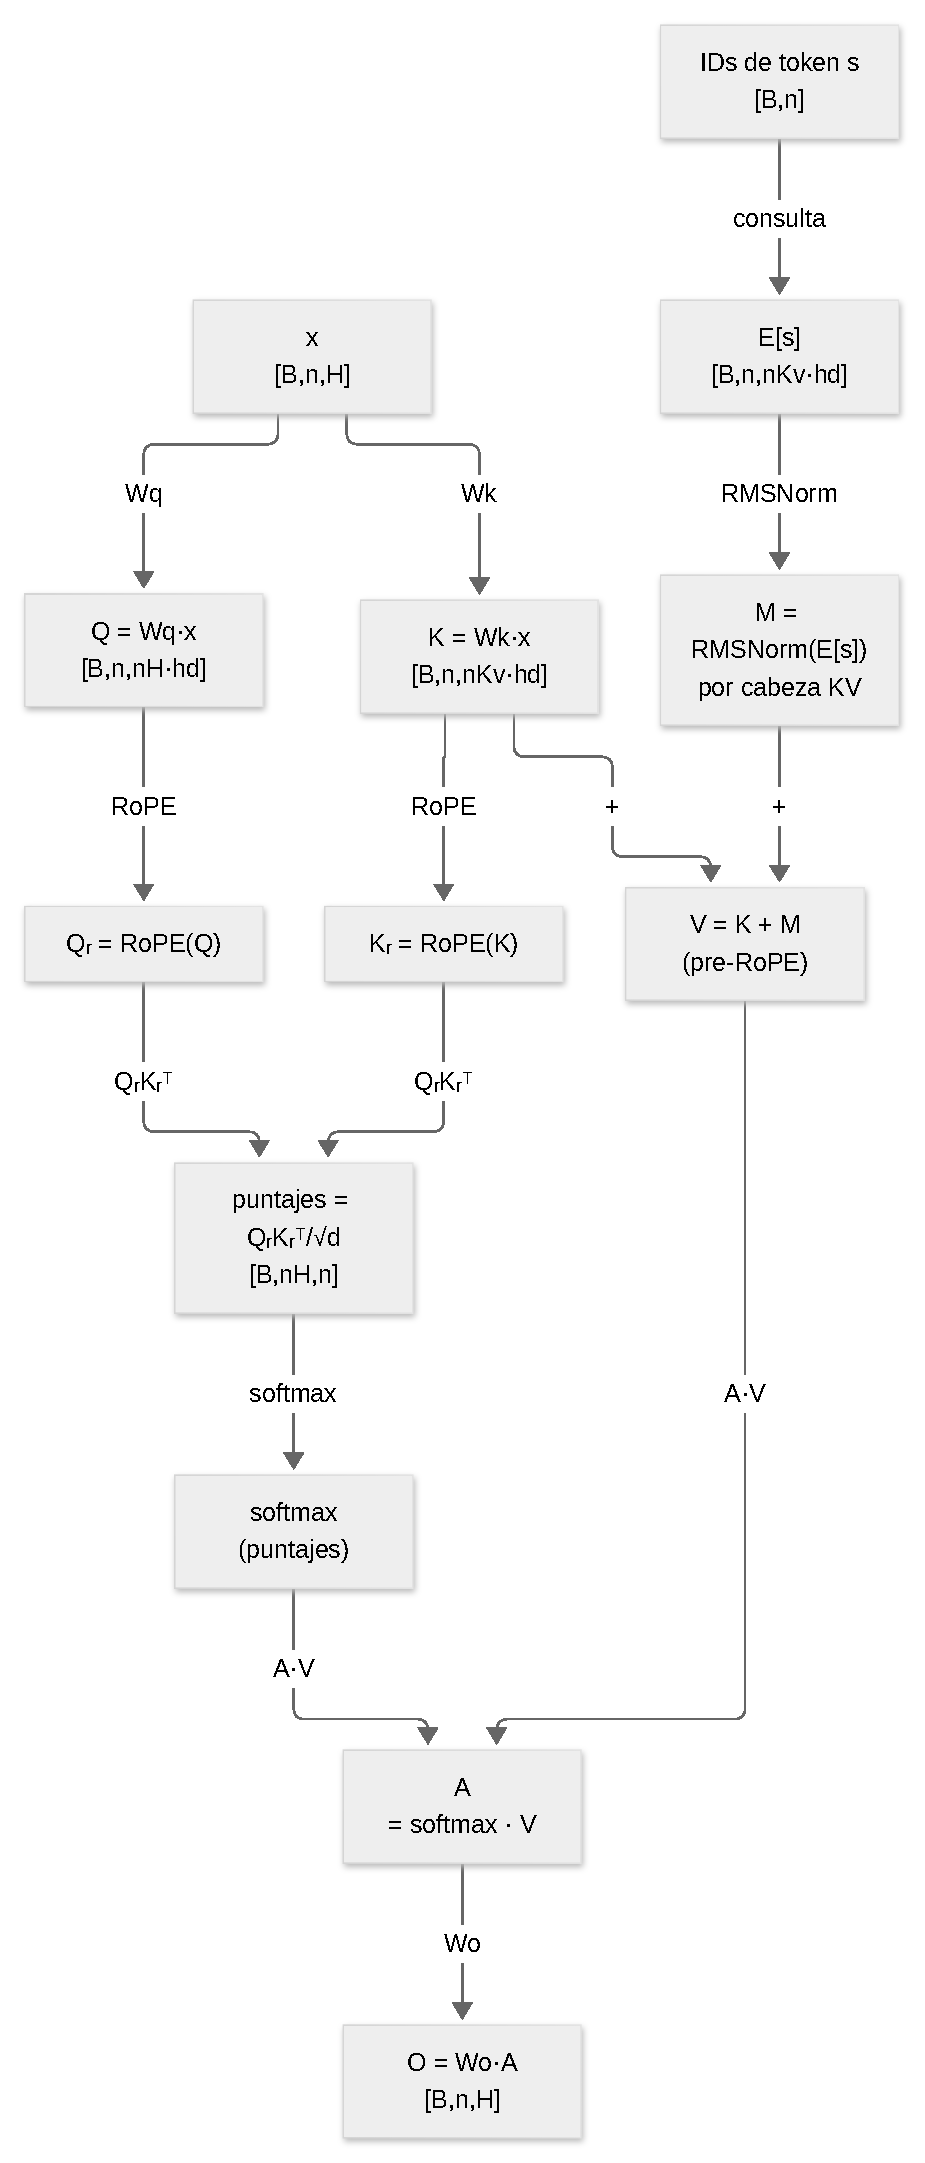
\includegraphics{../paper/figures/mixers/memory-es.pdf}}
\caption{Flujo de datos de Memory Attention: se elimina la proyección de valores;
los valores son las claves sin rotar más una fila de la tabla de memoria por ID de
token, normalizada con RMSNorm por cabeza KV. RoPE se aplica solo al par de puntuación.}
\label{fig:mixer-memory}
\end{figure}

Memory Attention \citep{kang_memory_attention_2026} elimina la proyección de
valores dedicada y construye los valores a partir de las claves contextuales más
la memoria específica de capa indexada por token. Con IDs de token $s$, tamaño de
vocabulario $N$ y $d_v = H_{KV} d_h$:

\begin{algorithmic}[1]
\State \textbf{Entrada:} estados ocultos $X \in \mathbb{R}^{T \times d}$, IDs de token $s$, tabla $E \in \mathbb{R}^{N \times d_v}$
\State $M \gets \mathrm{Norm}(E[s]) \in \mathbb{R}^{T \times d_v}$ \Comment{RMSNorm por vector de token, por cabeza clave/valor}
\State $Q \gets X W_Q$, \quad $K \gets X W_K$, \quad $V \gets K + M$ \Comment{sin $W_V$; valores desde claves sin rotar}
\State $Q_R \gets \mathrm{RoPE}(Q)$, \quad $K_R \gets \mathrm{RoPE}(K)$ \Comment{rotación solo para puntuar}
\State \textbf{Salida:} $Y = \mathrm{softmax}\!\left(\tfrac{Q_R K_R^\top}{\sqrt{d_k}} + C\right) V$
\end{algorithmic}

La salida se descompone como $O_{\mathrm{MA}} = A(K{+}M) = AK + AM$: un término de
recuperación contextual sobre las claves y un término de recuperación de memoria
agregado bajo la misma distribución de atención. A través de $L$ capas
reemplazadas, MA cambia los $L\,d\,d_v$ parámetros estándar de la proyección de
valores por $L(N d_v + p_{\mathrm{norm}})$ parámetros de memoria y normalización
---capacidad adicional accedida por búsqueda en lugar de cómputo denso. En
inferencia, la normalización por fila se pliega en la tabla ($E[i] \gets
\mathrm{Norm}(E[i])$), reduciendo la construcción de valores en línea a búsqueda
y suma, manteniendo un caché KV convencional. El artículo reporta mejor perplejidad
en LAMBADA/WikiText y precisión promedio en tareas posteriores para backbones
MHA/GQA/MQA con presupuestos de tokens igualados, con eficiencia de tokens
$1.42\times$/$1.16\times$; la comparación incluye los parámetros de memoria
adicionales, por lo que no aísla la estructura de la capacidad. MA-Offload
(tablas residentes en CPU con prefetch) y MA-Recall (reconstruir valores
históricos como $V_{1:T} = K_{1:T} + E[s_{1:T}]$ para un caché de valores
${\sim}50\%$ menor) se analizan pero no se implementan aquí.

\begin{itemize}[leftmargin=*]
    \item \textbf{Complejidad de entrenamiento}: $\mathcal{O}(n^2 d)$ de atención con
    construcción de valores $\mathcal{O}(n d_v)$ (búsqueda+norma+suma), en lugar de
    la proyección $\mathcal{O}(n\, d\, d_v)$.
    \item \textbf{Complejidad de inferencia}: $\mathcal{O}(n)$ por token con un
    caché KV convencional; $N d_v$ parámetros extra por capa.
    \item \textbf{Fortalezas}: Capacidad adicional sin crecimiento del cómputo
    denso; representaciones de token específicas por capa; agregación de atención
    estándar exacta; compatible con el caché KV por construcción.
    \item \textbf{Debilidades}: El número de parámetros crece con el vocabulario
    ($N \gg d$); requiere IDs de token (solo texto); las ganancias reportadas no
    están igualadas en parámetros.
\end{itemize}

\subsection{Arquitecturas Recurrentes y Retentivas}

\subsubsection{Redes Retentivas (RetNet)}

\begin{figure}[H]
\centering
\fitfigure{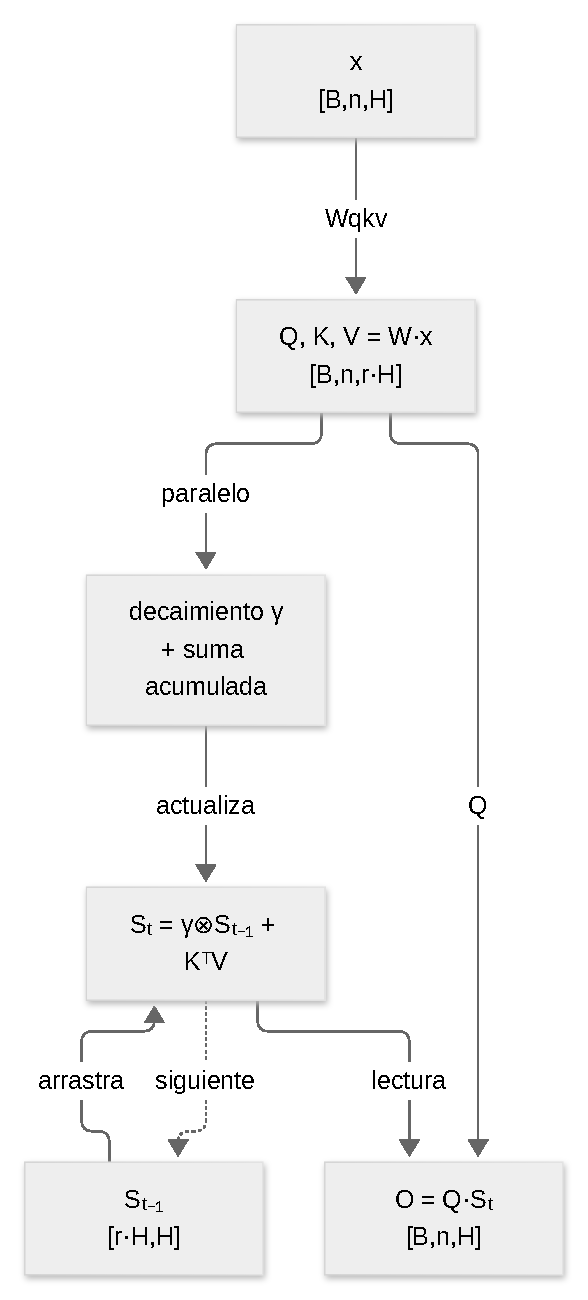
\includegraphics{../paper/figures/mixers/retnet-es.pdf}}
\caption{Flujo de datos de RetNet: proyecciones Q/K/V paralelas alimentan una recurrencia de estado con decaimiento; el estado se propaga entre pasos y la salida lo lee con la consulta.}
\label{fig:mixer-retnet}
\end{figure}
RetNet \citep{sun_retentive_2023} unifica tres paradigmas de cómputo: entrenamiento paralelo, inferencia recurrente y despliegue por fragmentos. Su innovación central es el \textbf{mecanismo de retención}, que utiliza una matriz de decaimiento exponencial fija para modelar la importancia temporal:

\begin{algorithmic}[1]
\State \textbf{Forma paralela (entrenamiento):}
\State $\text{matriz\_decaimiento}[i,j] \gets \gamma^{i-j}$ para $i \geq j$, si no $0$ \Comment{decaimiento exponencial causal}
\State $\text{matriz\_decaimiento}[i,j] \gets 0$ para $i < j$ \Comment{enmascaramiento causal}
\State $\mathbf{Y}_{\text{paralelo}} \gets (\mathbf{Q}\mathbf{K}^\top \odot \text{matriz\_decaimiento}) \mathbf{V}$ \Comment{multiplicación elemento a elemento con decaimiento}
\end{algorithmic}

\begin{algorithmic}[1]
\State \textbf{Forma recurrente (inferencia):}
\For{$t = 1, \ldots, n$}
    \State $\mathbf{s}_t \gets \gamma \mathbf{s}_{t-1} + \mathbf{k}_t \mathbf{v}_t^\top$ \Comment{actualización de estado con decaimiento}
    \State $\mathbf{y}_t \gets \mathbf{q}_t \mathbf{s}_t$ \Comment{salida mediante interacción consulta-estado}
\EndFor
\end{algorithmic}

El escalar de decaimiento $\gamma \in (0,1)$ controla la ventana temporal. RetNet utiliza \textbf{retención multi-escala} con diferentes valores de $\gamma$ por cabeza (ej., $\gamma = 1 - 2^{-5}, 1 - 2^{-6}, \ldots$), permitiendo dependencias a corto y largo plazo simultáneamente. El modo recurrente por fragmentos divide las secuencias en fragmentos, procesa cada fragmento en paralelo y enhebra un estado recurrente entre fragmentos.

\begin{itemize}[leftmargin=*]
    \item \textbf{Complejidad de entrenamiento}: $\mathcal{O}(n^2 \cdot d)$ (paralela), o $\mathcal{O}(n \cdot c \cdot d)$ (recurrente por fragmentos con tamaño de fragmento $c$).
    \item \textbf{Complejidad de inferencia}: $\mathcal{O}(1)$ por token, $\mathcal{O}(d^2)$ espacio de estado (matriz fija).
    \item \textbf{Fortalezas}: Inferencia en tiempo constante; triple paradigma de cómputo; consolidación multi-escala.
    \item \textbf{Debilidades}: El decaimiento fijo impone un sesgo inductivo rígido; puede truncar patrones de largo alcance aprendidos.
\end{itemize}

\subsubsection{Mamba: Modelos de Espacio de Estado Selectivos}

\begin{figure}[H]
\centering
\fitfigure{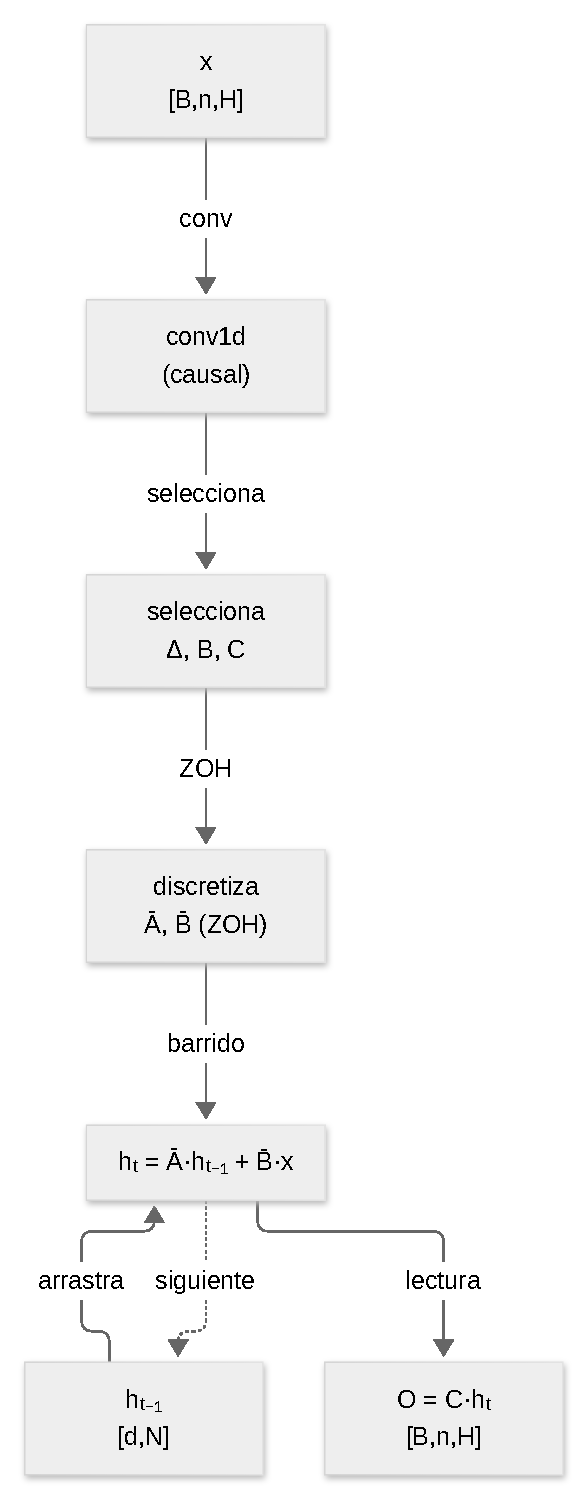
\includegraphics{../paper/figures/mixers/mamba-es.pdf}}
\caption{Flujo de datos de Mamba: una convolución causal alimenta selecciones de $\Delta$, $B$ y $C$ dependientes de la entrada, la discretización ZOH y un escaneo selectivo de espacio de estados cuyo estado se propaga entre pasos.}
\label{fig:mixer-mamba}
\end{figure}
Mamba \citep{gu_mamba_2023} enmarca la recurrencia como un sistema dinámico de tiempo continuo con parámetros dependientes de la entrada, logrando tanto entrenamiento lineal como inferencia en tiempo constante:

\begin{algorithmic}[1]
\State \textbf{Dinámica continua:} $h'(t) = \mathbf{A} h(t) + \mathbf{B} x(t)$, \quad $y(t) = \mathbf{C} h(t)$
\State \textbf{Discretización con tamaño de paso $\Delta_t$:}
\State $\bar{\mathbf{A}}_t \gets \exp(\Delta_t \mathbf{A})$
\State $\bar{\mathbf{B}}_t \gets (\Delta_t \mathbf{A})^{-1} (\exp(\Delta_t \mathbf{A}) - \mathbf{I}) \Delta_t \mathbf{B}_t$
\State \textbf{Actualización recurrente:}
\For{$t = 1, \ldots, n$}
    \State $\Delta_t \gets \text{softplus}(\text{Lineal}(x_t))$ \Comment{tamaño de paso dependiente de la entrada}
    \State $\mathbf{B}_t \gets \text{Lineal}(x_t)$, \quad $\mathbf{C}_t \gets \text{Lineal}(x_t)$ \Comment{matrices de proyección dependientes de la entrada}
    \State $h_t \gets \bar{\mathbf{A}}_t h_{t-1} + \bar{\mathbf{B}}_t x_t$ \Comment{transición de estado}
    \State $y_t \gets \mathbf{C}_t h_t$ \Comment{proyección de salida}
\EndFor
\end{algorithmic}

La innovación crítica es que $\mathbf{A}$ (la matriz del sistema) \textit{no} depende de la entrada, pero $\Delta_t$, $\mathbf{B}_t$ y $\mathbf{C}_t$ sí, haciendo que el sistema sea \textbf{variante en el tiempo}. Esta selectividad permite al modelo \textit{ignorar} información irrelevante estableciendo $\Delta_t$ cerca de cero, creando efectivamente una compuerta. Un algoritmo de escaneo paralelo consciente del hardware implementa la recurrencia eficientemente en GPUs fusionando el cómputo dentro de SRAM, evitando el costoso ancho de banda de HBM.

\begin{itemize}[leftmargin=*]
    \item \textbf{Complejidad de entrenamiento}: $\mathcal{O}(n \cdot d)$ mediante escaneo consciente del hardware (lineal en la longitud de la secuencia).
    \item \textbf{Complejidad de inferencia}: $\mathcal{O}(1)$ por token, $\mathcal{O}(d)$ estado (vector oculto).
    \item \textbf{Fortalezas}: Logra entrenamiento lineal e inferencia constante simultáneamente; práctico en secuencias largas (millones de tokens).
    \item \textbf{Debilidades}: La compresión del vector de estado puede debilitar la copia exacta y la recuperación asociativa densa en comparación con la atención completa.
\end{itemize}

\subsection{Transformers de Profundidad Continua: Integración EDO}

\subsubsection{Transformer EDO}

\begin{figure}[H]
\centering
\fitfigure{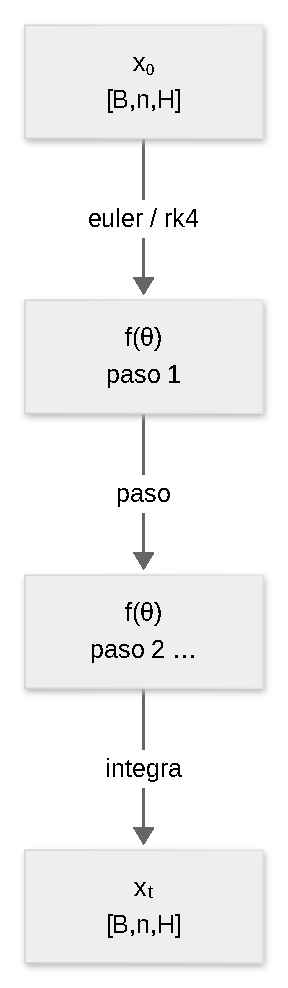
\includegraphics{../paper/figures/mixers/ode-es.pdf}}
\caption{Flujo de datos del bloque transformer EDO: el estado oculto se integra mediante uno o más pasos de Euler/RK4 antes de leer la salida.}
\label{fig:mixer-ode}
\end{figure}
El Transformer EDO \citep{zhang_continuous_2021} interpreta la profundidad de la red como integración numérica de un sistema dinámico continuo, utilizando solucionadores Runge-Kutta de orden superior para reducir el error de truncamiento:

\begin{algorithmic}[1]
\State \textbf{Formulación continua:} $\frac{dh(t)}{dt} = f_\theta(h(t), t)$ donde $f_\theta$ es la subred del transformer
\State \textbf{Aproximación discreta Runge-Kutta-4:}
\State $k_1 \gets f_\theta(h_t, t)$
\State $k_2 \gets f_\theta(h_t + \tfrac{1}{2}k_1, t + \tfrac{1}{2}\Delta t)$
\State $k_3 \gets f_\theta(h_t + \tfrac{1}{2}k_2, t + \tfrac{1}{2}\Delta t)$
\State $k_4 \gets f_\theta(h_t + k_3, t + \Delta t)$
\State $h_{t+1} \gets h_t + \frac{\Delta t}{6}(k_1 + 2k_2 + 2k_3 + k_4)$ \Comment{combinación ponderada}
\end{algorithmic}

En lugar de las conexiones residuales simples de Euler $h_{t+1} = h_t + f_\theta(h_t)$, el bloque RK4 calcula cuatro evaluaciones intermedias y las combina con los pesos clásicos de RK4. Para evitar gradientes que se desvanecen, la arquitectura introduce \textbf{compuertas aprendidas} que interpolan entre aproximaciones intermedias:

\begin{algorithmic}[1]
\State $g \gets \sigma(\text{Lineal}([k_1, k_2, k_3, k_4]))$ \Comment{compuerta aprendible}
\State $h_{t+1} \gets h_t + g \cdot k_1 + (1-g) \cdot k_2$ \Comment{refinamiento interpolado}
\end{algorithmic}

Esta formulación reduce el número efectivo de parámetros mediante el uso compartido de pesos---la misma $f_\theta$ se evalúa múltiples veces---proporcionando un refinamiento de trayectoria más rico.

\begin{itemize}[leftmargin=*]
    \item \textbf{Complejidad de entrenamiento}: $\mathcal{O}(k \cdot n^2 \cdot d)$ donde $k$ es el orden RK (4 para RK4).
    \item \textbf{Complejidad de inferencia}: $\mathcal{O}(k \cdot n)$ por token (mayor sobrecarga constante).
    \item \textbf{Fortalezas}: Precisión significativamente mayor en tareas de generación (BLEU de última generación); eficiente en parámetros mediante uso compartido de pesos.
    \item \textbf{Debilidades}: Alto costo de cómputo por paso; la latencia de inferencia aumenta por un factor constante $k$; requiere compuertas complejas para la estabilidad.
\end{itemize}

\subsection{Memoria en Tiempo de Prueba: Titans}

\begin{figure}[H]
\centering
\fitfigure{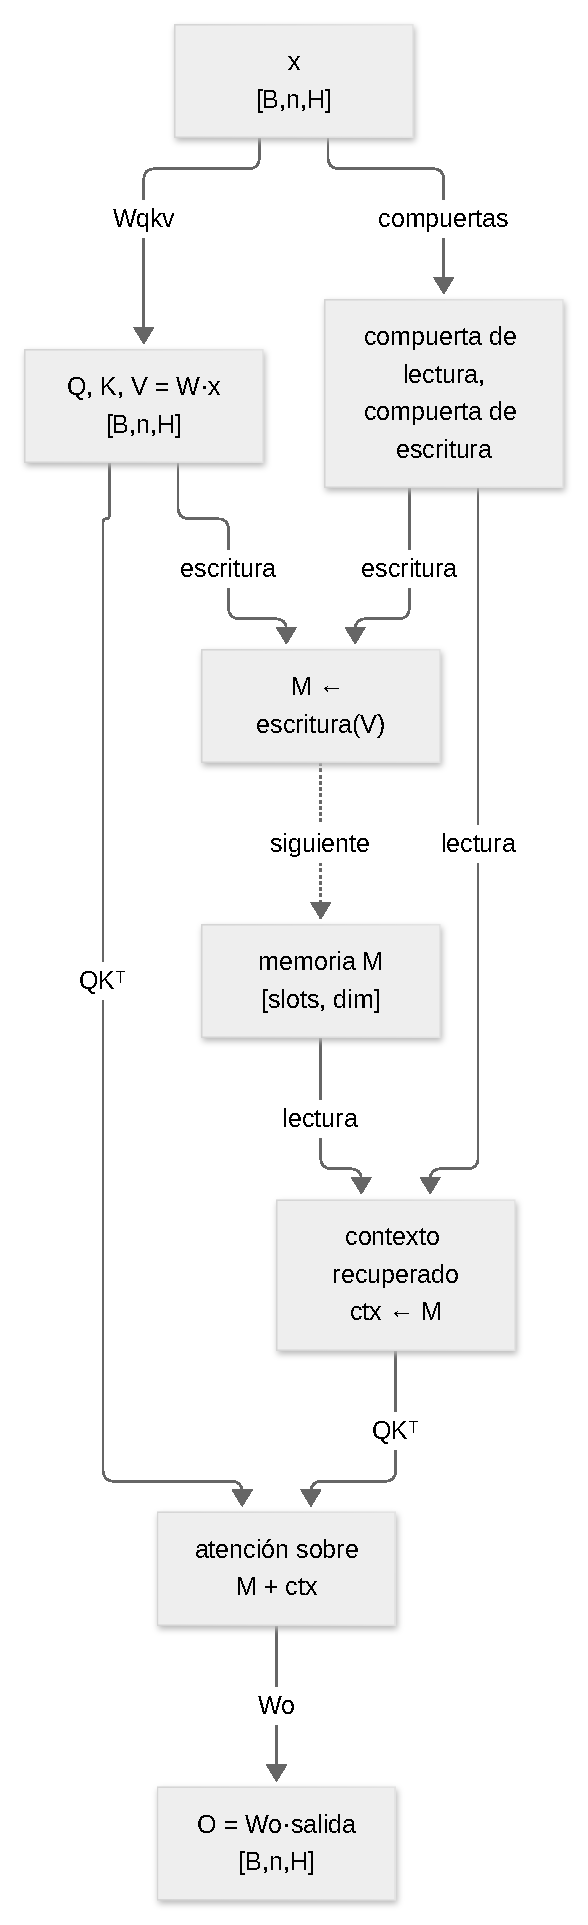
\includegraphics{../paper/figures/mixers/titan-es.pdf}}
\caption{Flujo de datos de la memoria en tiempo de prueba de Titans: la atención densa Q/K/V opera sobre una ventana local mientras compuertas de lectura y escritura actualizan una memoria asociativa que se propaga entre pasos.}
\label{fig:mixer-titan}
\end{figure}

La arquitectura Titans \citep{behrouz_titans_2025} introduce una dimensión ortogonal: en lugar de pesos estáticos, el modelo mantiene una memoria aprendible que se \textit{actualiza durante la inferencia} basada en una señal impulsada por sorpresa:

\begin{algorithmic}[1]
\State \textbf{Atención local a corto plazo:} Aplicar atención estándar o dispersa dentro de una ventana de contexto fija $c$
\State $y_t^{\text{local}} \gets \text{Atencion}(q_t, k_{[t-c:t]}, v_{[t-c:t]})$
\State \textbf{Señal de actualización de memoria (sorpresa):}
\State $S_t \gets \eta_t S_{t-1} - \theta_t \nabla_\ell(\mathcal{M}_{t-1}; x_t)$ \Comment{sorpresa como gradiente de la pérdida respecto a la memoria}
\State $\mathcal{M}_t \gets (1 - \alpha_t) \mathcal{M}_{t-1} + S_t$ \Comment{memoria actualizada mediante EMA}
\State \textbf{Recuperación de memoria a largo plazo:}
\State $y_t^{\text{memoria}} \gets \mathcal{M}_t^* (q_t)$ \Comment{consultar módulo de memoria para información recuperada}
\State \textbf{Combinación de salida:}
\State $y_t \gets y_t^{\text{local}} + \text{compuerta}(y_t^{\text{memoria}})$ \Comment{combinar memoria local y recuperada}
\end{algorithmic}

El módulo de memoria $\mathcal{M}$ se actualiza literalmente durante el paso hacia adelante calculando gradientes de una pérdida asociativa y aplicando pasos de SGD con momento. Las tasas de decaimiento $\eta_t, \theta_t, \alpha_t$ son en sí mismas dependientes de la entrada, permitiendo al modelo cambiar de paradigma de memoria cuando el contexto cambia.

\begin{itemize}[leftmargin=*]
    \item \textbf{Complejidad de entrenamiento}: Aproximadamente $\mathcal{O}(c^2 + n \cdot f)$ donde $c$ es la ventana local y $f$ es la sobrecarga de actualización de memoria.
    \item \textbf{Complejidad de inferencia}: $\mathcal{O}(c^2)$ atención local más $\mathcal{O}(1)$ recuperación de memoria por token.
    \item \textbf{Fortalezas}: Maneja longitudes de contexto extremas; permite recuperación asociativa real; la memoria se adapta a la entrada.
    \item \textbf{Debilidades}: Significativamente más complejo; la inferencia incluye cálculos de gradientes; mayor sobrecarga de coordinación.
\end{itemize}

\subsection{Despacho de Mezclador Guiado por Patrón}

El código base selecciona un mezclador por bloque a partir del \texttt{layer\_pattern} configurado. La lógica de despacho enruta los bloques dispersos en tiempo de inferencia (\texttt{fasa}, \texttt{sparge}) a atención estándar densa mientras el modelo está en modo entrenamiento, y a su implementación dispersa durante la evaluación; el resto de bloques se enruta a la implementación de familia correspondiente.

\begin{algorithm}[t]
\caption{Paso Adelante del Mezclador Guiado por Patrón (Conceptual)}
\begin{algorithmic}[1]
\Require Estados ocultos $H$, patrón $P$, índice de capa $\ell$
\State $m \gets P[\ell \bmod |P|]$
\If{$m \in \{\texttt{fasa}, \texttt{sparge}\}$ y el modelo está en modo entrenamiento}
    \State $H \gets \text{softmax-attention}(H)$ \Comment{atención densa sustituta, mismas proyecciones}
\ElsIf{$m=\texttt{standard}$}
    \State $H \gets \text{softmax-attention}(H)$
\ElsIf{$m=\texttt{ca}$}
    \State $H \gets \text{atención-continua}(H)$ \Comment{integración exacta por tramos}
\ElsIf{$m=\texttt{sigmoid}$}
    \State $H \gets \text{sigmoid-attention}(H)$
\ElsIf{$m=\texttt{memory}$}
    \State $H \gets \text{memory-attention}(H)$
\ElsIf{$m=\texttt{retnet}$}
    \State $H \gets \text{retention}(H)$
\ElsIf{$m=\texttt{mamba}$}
    \State $H \gets \text{selective-ssm}(H)$
\ElsIf{$m=\texttt{ode}$}
    \State $H \gets \text{rk-step}(H)$
\ElsIf{$m$ es una clave de atención dispersa}
    \State $H \gets \text{sparse-attention-family}(H)$
\ElsIf{$m$ es una clave de atención con compuerta}
    \State $H \gets \text{gated-attention-family}(H)$
\Else
    \State $H \gets \text{memory-augmented-attn}(H)$
\EndIf
\State \Return $H$
\end{algorithmic}
\end{algorithm}

El campo exhibe una progresión clara a lo largo de dos ejes: (i) \textbf{eficiencia computacional}, pasando de $O(n^2)$ a $O(n)$ u $O(1)$, y (ii) \textbf{adaptabilidad de memoria}, pasando de pesos estáticos a modelos dinámicos actualizados en tiempo de prueba. La atención estándar sigue siendo la línea base de expresividad; Mamba y RetNet representan la frontera práctica de eficiencia; Titans introduce un eje de innovación ortogonal (aprendizaje en tiempo de prueba). La elección de arquitectura refleja la restricción fundamental de ingeniería: expresividad versus costo de despliegue. La familia de atención latente, que comprime el caché KV en un latente de rango bajo, se cubre en el Apéndice~\ref{sec:annex-latent}.